\documentclass[journal]{IEEEtran}
\ifCLASSINFOpdf
\usepackage[pdftex]{graphicx}
\else
\fi
\usepackage{amsmath}
\usepackage{amssymb}
\usepackage{amsthm}
\usepackage{bm}
\usepackage{mathrsfs}
\hyphenation{La-grange La-grang-ian dy-nam-ics}
\newcommand{\bma}[1]{\left[\begin{array}{#1}}
\newcommand{\ema}{\end{array}\right]}
\newcommand{\trans}{{\ensuremath{\mathsf{T}}}} % transpose
\newcommand{\utimes}{ {\raisebox{-0.6ex}{ \kern-1.0ex\raisebox{0.6ex}{ \small $\mathsf{v}$}}} } % 
\newcommand{\onehalf}{\mbox{$\textstyle{\frac{1}{2}}$}}
\DeclareMathAlphabet{\mbf}{OT1}{ptm}{b}{n}
\newcommand{\mbs}[1]{{\boldsymbol{#1}}}
\newcommand{\mbfbar}[1]{{\bar{\mbf{#1}}}}
\newcommand{\mbfhat}[1]{{\hat{\mbf{#1}}}}
\newcommand{\mbftilde}[1]{{\tilde{\mbf{#1}}}}
\newcommand{\mbsbar}[1]{{\bar{\boldsymbol{#1}}}}
\newcommand{\mbshat}[1]{{\hat{\boldsymbol{#1}}}}
\newcommand{\mbstilde}[1]{{\tilde{\boldsymbol{#1}}}}
\newcommand{\pspace}{\mathbb{P}} 
\newcommand{\ura}[1]{{\underrightarrow{{#1}}}}
\newcommand{\vectrix}[1]{\ensuremath \underrightarrow{\boldsymbol{\mathcal{F}}}_{#1}}
\def\fdota{{\raisebox{-2pt}{\LARGE $\cdot$}}}
\def\fdotb{{\raisebox{-0.6ex}{ \kern0.2ex\raisebox{0.8ex}{\tiny $\hspace*{-1ex}\circ$}}}}
\def\fddota{{\raisebox{-2pt}{\LARGE $\cdot\hspace*{-0.2ex}\cdot$}}}
\def\fddotb{{\raisebox{-0.6ex}{ \kern0.2ex\raisebox{0.8ex}{\tiny $\hspace*{-1ex}\circ\circ$}}}}
\newcommand{\fdot}[1]{{^{\fdota{\mbox{\footnotesize${#1}$}}}}}
\newcommand{\fddot}[1]{{^{\fddota{\mbox{\footnotesize${#1}$}}}}}
\newcommand{\beq}{\begin{equation}}
\newcommand{\eeq}{\end{equation}}
\newcommand{\bdis}{\begin{displaymath}}
\newcommand{\edis}{\end{displaymath}}
\newcommand{\beqarray}{\begin{eqnarray}}
\newcommand{\eeqarray}{\end{eqnarray}}
\newcommand{\beqarraynn}{\begin{eqnarray*}}
\newcommand{\eeqarraynn}{\end{eqnarray*}}

\begin{document}

\title{Quad-Rotor Helicopter Kinematics}

\author{{Gregory Miller 50760004}}

\markboth{AER 540 -- Intermediate Dynamics, Fall 2014}
{}

\maketitle

\begin{abstract}
This document provides a brief introduction to quad-rotor helicopters and then computes the kinematics of a quad-rotor helicopter, knowledge that the helicopter will need to fly itself through a set course.   
\end{abstract}

\IEEEpeerreviewmaketitle

\section{Introduction and Motivation}
\label{sec:intro_section}

\IEEEPARstart{A}{}quad-rotor helicopter is a flying device that has four horizontal spinning rotors which produce the upward thrust needed to life the center piece, or body of the helicopter, into the air. See Figure \ref{fig:quad_intro} below, courtesy of website \cite{quad_intro}, for a visual example of a quad-rotor helicopter:

\begin{figure}[ht]
    \centering
        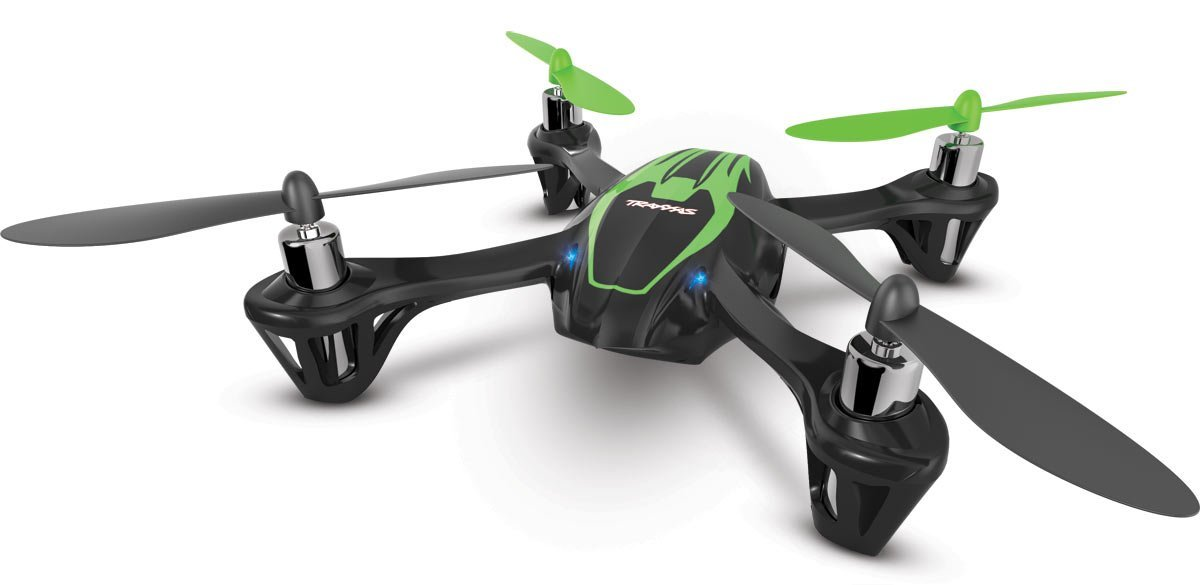
\includegraphics[width=.30\textwidth]{quad_intro}
    \caption{A visual example of a quad-rotor helicopter. Notice the four rotors.}
    \label{fig:quad_intro}
\end{figure}

 The purpose of this course project is to analyze the kinematics and dynamics of a quad-rotor helicopter as it flies through a pre-determined flight path. The inspiration for this project came from the Michigan Autonomous Aerial Vehicles Club (MAAV). Every year,
 the club designs and constructs a quad-rotor helicopter to compete in a competition the subsequent August. In this competition, the goal is to have the quad-rotor helicopter autonomously navigate its own way through an obstacle course. As no human navigation input into the helicopter is allowed, its processor must use controllers
 that can successfully command the helicopter's actuators, i.e., the four spinning rotors, to direct the helicopter through its path. As such, it would be useful to model the quad-rotor helicopter's kinematics as this information is needed in order to design the controllers to produce steady and stable flight through the
 obstacle course.   

\section{Kinematics of the Quad-Rotor Helicopter}
\label{sec:kinematics_section}

Kinematics refers to the geometry of motion of a moving object. The motion of the quad-rotor helicopter is going to be determined by the locations and directions of the external forces that are applied to its body. Arguably the most important of these forces are the four thrust forces produced by the helicopter's four rotors. These forces lift the helicopter into the air and propel it forward. In fact, the only means in which the helicopter has control over its motion is through its knowledge of the locations of these forces and its orientation in space. As such, knowing the kinematics of the four rotors is necessary. Figure \ref{fig:helicopterkin} below shows the relevant kinematics information for the helicopter from a top-down perspective:

\begin{figure}[ht]
    \centering
        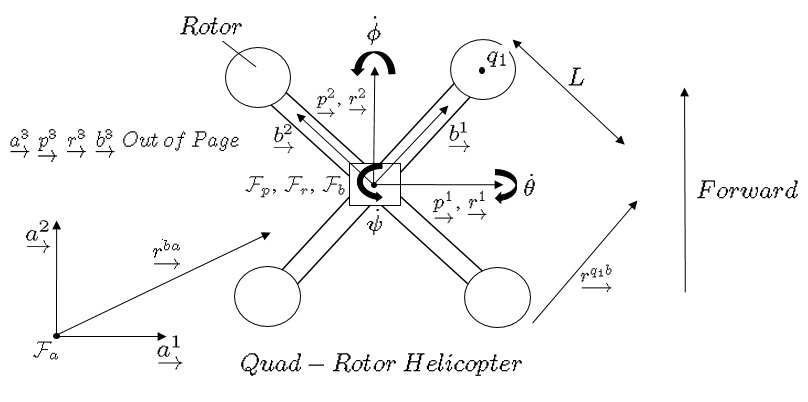
\includegraphics[width=.50\textwidth]{helicopterkin}
    \caption{The relevant kinematics information for the quad-rotor helicopter}
    \label{fig:helicopterkin}
\end{figure}

\pagebreak
Note point $q_1$ located on the upper-right rotor in Figure \ref{fig:helicopterkin}. The goal is to compute the kinematics of the four rotors, i.e., $\underrightarrow{v^{q_1a/a}}$, the velocity, and $\underrightarrow{a^{q_1a/a}}$, the acceleration. To begin, there are four frames shown in Figure \ref{fig:helicopterkin}. They are summarized in the following list:

\begin{enumerate}
\item An inertial frame $\mathcal{F}_a$. This frame remains fixed to the ground. 
\item The pitch (p) frame $\mathcal{F}_p$. This frame is created by rotating $\mathcal{F}_a$ about $\underrightarrow{a^1}$ by the angle $\theta$. This frame is coincident with the quad-rotor helicopter body and the basis vector $\underrightarrow{p^2}$ remains fixed in the plane created by the four rotors.
\item The roll (r) frame $\mathcal{F}_r$. This frame is created by rotating $\mathcal{F}_p$ about $\underrightarrow{p^2}$ by the angle $\phi$. This frame is coincident with the quad-rotor helicopter body and the basis vector $\underrightarrow{r^1}$ remains fixed in the plane created by the four rotors.
\item The yaw, or body (b), frame $\mathcal{F}_b$. This frame is created by rotating $\mathcal{F}_r$ about $\underrightarrow{r^3}$ by the angle $\psi$. This frame is fixed to the quad-rotor helicopter body and the basis vectors $\underrightarrow{b^1}$ and $\underrightarrow{b^2}$ remain parallel to the helicopter's arms. 
\end{enumerate}

For the Direction-Cosine Matrix (DCM) representation, Euler-angle rotation matrices will be used because they are well-suited for the pitch-roll-yaw frame designations described above and because the quad-rotor helicopter is never expected to produce the kinematic singularity associated with Euler-angle rotation matrices, or in other words, rotate $90$ degrees about any one axis. 

That being said, the four frames undergo a 1-2-3 Euler-angle sequence. Equation \ref{eq:eulerseq} below provides the formal representation of this sequence:

\begin{equation}
	\mathcal{F}_a \xrightarrow[\underline{C_1(\theta)}]{} \mathcal{F}_p \xrightarrow[\underline{C_2(\phi)}]{} \mathcal{F}_r \xrightarrow[\underline{C_3(\psi)}]{} \mathcal{F}_b
	\label{eq:eulerseq}
\end{equation}

The overall DCM matrix is computed next in Equations \ref{eq:dcmbase} and \ref{eq:dcm}:

\begin{equation}
	\underline{C_{ba}}=\underline{C_{br}}\underline{C_{rp}}\underline{C_{pa}}=\underline{C_3{(\psi)}}\underline{C_2{(\phi)}}\underline{C_1{(\theta)}}
	\label{eq:dcmbase}
\end{equation}
\begin{equation}
	\underline{C_{ba}}=\left( \begin{array}{ccc}
	c_{\phi}c_{\psi} & c_{\theta}s_{\psi}+s_{\theta}s_{\phi}c_{\psi} & s_{\theta}s_{\psi}-c_{\theta}s_{\phi}c_{\psi} \\
	-c_{\phi}s_{\psi} & c_{\theta}c_{\psi}-s_{\theta}s_{\phi}s_{\psi} & s_{\theta}c_{\psi}+c_{\theta}s_{\phi}s_{\psi} \\
	s_{\phi} & -s_{\theta}c_{\phi} & c_{\theta}c_{\phi} \\
	\end{array} \right)
	\label{eq:dcm}
\end{equation}

Next, the angular velocity of $\mathcal{F}_b$ with respect to $\mathcal{F}_a$, $\underrightarrow{\omega^{ba}}$, is computed. Note that angular velocities of the frames with respect to each other add, as stated in Equation \ref{eq:angadd}:

\begin{equation}
	\underrightarrow{\omega^{ba}}=\underrightarrow{\omega^{br}}+\underrightarrow{\omega^{rp}}+\underrightarrow{\omega^{pa}}
	\label{eq:angadd}
\end{equation}

Using Poisson's Equation, Equation \ref{eq:poisson}, the following can be stated concerning the components of three angular velocities on the right-hand side of Equation \ref{eq:angadd}, stated in Equations \ref{eq:angcomp1} through \ref{eq:angcomp3}:

\begin{equation}
	\underline{\dot{C_{yx}}}=-\underline{\omega^{yx\times}_y}\underline{C_{yx}}
	\label{eq:poisson}
\end{equation}
\begin{equation}
	\underline{\dot{C_1(\theta)}}=-\dot{\theta}\underline{\mathbf{1}^{\times}_1}\underline{C_1(\theta)} \xrightarrow[]{} \underline{\omega^{pa}_p}=\dot{\theta}\underline{\mathbf{1}_1}
	\label{eq:angcomp1}
\end{equation}
\begin{equation}
	\underline{\dot{C_2(\phi)}}=-\dot{\phi}\underline{\mathbf{1}^{\times}_2}\underline{C_2(\phi)} \xrightarrow[]{} \underline{\omega^{rp}_r}=\dot{\phi}\underline{\mathbf{1}_2}
	\label{eq:angcomp2}
\end{equation}
\begin{equation}
	\underline{\dot{C_3(\psi)}}=-\dot{\psi}\underline{\mathbf{1}^{\times}_3}\underline{C_3(\psi)} \xrightarrow[]{} \underline{\omega^{br}_b}=\dot{\psi}\underline{\mathbf{1}_3}
	\label{eq:angcomp3}
\end{equation}

Adding the angular velocity components together and resolving the results in $\mathcal{F}_b$ in Equations \ref{eq:angaddresb1} through \ref{eq:angaddresb3} to obtain an explicit expression for $\underrightarrow{\omega^{ba}}$:

\begin{equation}
	\underrightarrow{\omega^{ba}}=\underrightarrow{\mathcal{F}^T_b}\underline{\omega^{br}_b}+\underrightarrow{\mathcal{F}^T_r}\underline{\omega^{rp}_r}+\underrightarrow{\mathcal{F}^T_p}\underline{\omega^{pa}_p}
	\label{eq:angaddresb1}
\end{equation}
\begin{equation}
\underrightarrow{\omega^{ba}}=\underrightarrow{\mathcal{F}^T_b}[\dot{\psi}\underline{\mathbf{1}_3}+\underline{C_3(\psi)}\dot{\phi}\underline{\mathbf{1}_2}+\underline{C_3(\psi)}\underline{C_2(\phi)}\dot{\theta}\underline{\mathbf{1}_1}]
\label{eq:angaddresb2}
\end{equation}
\begin{equation}
\underrightarrow{\omega^{ba}}=\underrightarrow{\mathcal{F}^T_b}
	\left( \begin{array}{c}
	c_{\phi}c_{\psi}\dot{\theta}+s_{\psi}\dot{\phi}  \\
	-c_{\phi}s_{\psi}\dot{\theta}+c_{\psi}\dot{\phi}  \\
	s_{\phi}\dot{\theta}+\dot{\psi} \\
	\end{array} \right)
\label{eq:angaddresb3}
\end{equation}

Next, as is clear in Figure \ref{fig:helicopterkin}, the following position vector relation, Equation \ref{eq:posvect}, holds:

\begin{equation}
	\underrightarrow{r^{q_1a}}=	\underrightarrow{r^{ba}}+	\underrightarrow{r^{q_1b}}
	\label{eq:posvect}
\end{equation}

Noting that the positions $x_b$, $y_b$, and $z_b$, which are not constant, locate point $b$ with respect to point $a$, and that $L$, which is constant, locates point $q_1$ with respect to point $b$ parallel to the $\underrightarrow{b^1}$ axis, Equation \ref{eq:posvectcomp} provides the components of the two position vectors on the right-hand side of Equation \ref{eq:posvect}:

\begin{equation}
	\underrightarrow{r^{q_1a}}=\underrightarrow{\mathcal{F}^T_a}
		\left( \begin{array}{c}
		x_b \\
		y_b \\
		z_b \\
		\end{array} \right)+\underrightarrow{\mathcal{F}^T_b}
				\left( \begin{array}{c}
				L \\
				0 \\
				0 \\
				\end{array} \right)			
	\label{eq:posvectcomp}
\end{equation}

Next, the velocity $\underrightarrow{v^{q_1a/a}}$ is computed in Equations \ref{eq:vel1} through \ref{eq:vel5}. Note the use of the Transport Theorem, the angular velocity $\underrightarrow{\omega^{ba}}$ stated in Equation \ref{eq:angaddresb3}, and the fact that $L$ is constant:

\begin{equation}
	\underrightarrow{v^{q_1a/a}}=\underrightarrow{r^{q_1a\cdot{a}}}=\underrightarrow{r^{ba\cdot{a}}}+\underrightarrow{r^{q_1b\cdot{a}}}
	\label{eq:vel1}
\end{equation}
\begin{equation}
	\underrightarrow{v^{q_1a/a}}=\underrightarrow{\mathcal{F}^T_a}\underline{\dot{r^{ba}_a}}+\underrightarrow{r^{q_1b\cdot{b}}}+	\underrightarrow{\omega^{ba}}\times\underrightarrow{r^{q_1b}}
	\label{eq:vel2}
\end{equation}
\begin{equation}
	\underrightarrow{v^{q_1a/a}}=\underrightarrow{\mathcal{F}^T_a}\left( \begin{array}{c}
			\dot{x_b} \\
			\dot{y_b} \\
			\dot{z_b} \\
			\end{array} \right)+\underrightarrow{\mathcal{F}^T_b}\underline{0}+\underrightarrow{\mathcal{F}^T_b}\underline{\omega^{ba\times}_b}\underline{r^{ba}_b}
	\label{eq:vel3}
\end{equation}
\begin{equation}
	\underrightarrow{v^{q_1a/a}}=\underrightarrow{\mathcal{F}^T_b}\underline{C_{ba}}\left( \begin{array}{c}
			\dot{x_b} \\
			\dot{y_b} \\
			\dot{z_b} \\
			\end{array} \right)+\underrightarrow{\Delta}		
	\label{eq:vel4}
\end{equation}
\begin{equation}
	\underrightarrow{\Delta}=\underrightarrow{\mathcal{F}^T_b}\left(    \begin{array}{c}
						0 \\
			(s_{\phi}\dot{\theta}+\dot{\psi})L \\
			(c_{\phi}s_{\psi}\dot{\theta}-c_{\psi}\dot{\phi})L \\
						\end{array} \right)		
	\label{eq:vel5}
\end{equation}
Note that $\underline{C_{ba}}$ was provided in Equation \ref{eq:dcm}. Last, the acceleration $\underrightarrow{a^{q_1a/a}}$ is computed in Equations \ref{eq:acc1} and \ref{eq:acc2}. Note the use of the Transport Theorem and the angular velocity $\underrightarrow{\omega^{ba}}$ stated in Equation \ref{eq:angaddresb3}:

\begin{equation}
	\underrightarrow{a^{q_1a/a}}=\underrightarrow{v^{q_1a/a\cdot{a}}}=\underrightarrow{\mathcal{F}^T_a}\underline{\ddot{r^{ba}_a}}+\underrightarrow{\Delta^{\cdot{a}}}
	\label{eq:acc1}
\end{equation}
\begin{equation}
	\underrightarrow{a^{q_1a/a}}=\underrightarrow{\mathcal{F}^T_b}\underline{C_{ba}}\left( \begin{array}{c}
				\ddot{x_b} \\
				\ddot{y_b} \\
				\ddot{z_b} \\
				\end{array} \right)+\underrightarrow{\mathcal{F}^T_b}(\underline{\dot{\Delta_b}}+\underline{\omega^{ba\times}_b}\underline{\Delta_b})
	\label{eq:acc2}
\end{equation}

Computing the acceleration, the calculations of which are too cumbersome to write into this document, produces $\ddot{\theta}$, $\ddot{\phi}$, and $\ddot{\psi}$ terms. Note that $L$ is constant.

\section{Conclusion}
In this document, a brief quad-rotor helicopter introduction was provided along with the reasoning behind modeling its kinematics for use in a self-guided obstacle course. After, the overall DCM matrix, the angular velocity, and the relevant positions, velocities, and accelerations were computed. The next step in the process is to model the dynamics of the quad-rotor helicopter so that its equations of motion can be determined. 

\bibliographystyle{IEEEtran}
\bibliography{540_refs}

\end{document}


